% Options for packages loaded elsewhere
\PassOptionsToPackage{unicode}{hyperref}
\PassOptionsToPackage{hyphens}{url}
\PassOptionsToPackage{dvipsnames,svgnames,x11names}{xcolor}
%
\documentclass[
  letterpaper,
  DIV=11,
  numbers=noendperiod]{scrreprt}

\usepackage{amsmath,amssymb}
\usepackage{iftex}
\ifPDFTeX
  \usepackage[T1]{fontenc}
  \usepackage[utf8]{inputenc}
  \usepackage{textcomp} % provide euro and other symbols
\else % if luatex or xetex
  \usepackage{unicode-math}
  \defaultfontfeatures{Scale=MatchLowercase}
  \defaultfontfeatures[\rmfamily]{Ligatures=TeX,Scale=1}
\fi
\usepackage{lmodern}
\ifPDFTeX\else  
    % xetex/luatex font selection
\fi
% Use upquote if available, for straight quotes in verbatim environments
\IfFileExists{upquote.sty}{\usepackage{upquote}}{}
\IfFileExists{microtype.sty}{% use microtype if available
  \usepackage[]{microtype}
  \UseMicrotypeSet[protrusion]{basicmath} % disable protrusion for tt fonts
}{}
\makeatletter
\@ifundefined{KOMAClassName}{% if non-KOMA class
  \IfFileExists{parskip.sty}{%
    \usepackage{parskip}
  }{% else
    \setlength{\parindent}{0pt}
    \setlength{\parskip}{6pt plus 2pt minus 1pt}}
}{% if KOMA class
  \KOMAoptions{parskip=half}}
\makeatother
\usepackage{xcolor}
\setlength{\emergencystretch}{3em} % prevent overfull lines
\setcounter{secnumdepth}{5}
% Make \paragraph and \subparagraph free-standing
\ifx\paragraph\undefined\else
  \let\oldparagraph\paragraph
  \renewcommand{\paragraph}[1]{\oldparagraph{#1}\mbox{}}
\fi
\ifx\subparagraph\undefined\else
  \let\oldsubparagraph\subparagraph
  \renewcommand{\subparagraph}[1]{\oldsubparagraph{#1}\mbox{}}
\fi

\usepackage{color}
\usepackage{fancyvrb}
\newcommand{\VerbBar}{|}
\newcommand{\VERB}{\Verb[commandchars=\\\{\}]}
\DefineVerbatimEnvironment{Highlighting}{Verbatim}{commandchars=\\\{\}}
% Add ',fontsize=\small' for more characters per line
\usepackage{framed}
\definecolor{shadecolor}{RGB}{241,243,245}
\newenvironment{Shaded}{\begin{snugshade}}{\end{snugshade}}
\newcommand{\AlertTok}[1]{\textcolor[rgb]{0.68,0.00,0.00}{#1}}
\newcommand{\AnnotationTok}[1]{\textcolor[rgb]{0.37,0.37,0.37}{#1}}
\newcommand{\AttributeTok}[1]{\textcolor[rgb]{0.40,0.45,0.13}{#1}}
\newcommand{\BaseNTok}[1]{\textcolor[rgb]{0.68,0.00,0.00}{#1}}
\newcommand{\BuiltInTok}[1]{\textcolor[rgb]{0.00,0.23,0.31}{#1}}
\newcommand{\CharTok}[1]{\textcolor[rgb]{0.13,0.47,0.30}{#1}}
\newcommand{\CommentTok}[1]{\textcolor[rgb]{0.37,0.37,0.37}{#1}}
\newcommand{\CommentVarTok}[1]{\textcolor[rgb]{0.37,0.37,0.37}{\textit{#1}}}
\newcommand{\ConstantTok}[1]{\textcolor[rgb]{0.56,0.35,0.01}{#1}}
\newcommand{\ControlFlowTok}[1]{\textcolor[rgb]{0.00,0.23,0.31}{#1}}
\newcommand{\DataTypeTok}[1]{\textcolor[rgb]{0.68,0.00,0.00}{#1}}
\newcommand{\DecValTok}[1]{\textcolor[rgb]{0.68,0.00,0.00}{#1}}
\newcommand{\DocumentationTok}[1]{\textcolor[rgb]{0.37,0.37,0.37}{\textit{#1}}}
\newcommand{\ErrorTok}[1]{\textcolor[rgb]{0.68,0.00,0.00}{#1}}
\newcommand{\ExtensionTok}[1]{\textcolor[rgb]{0.00,0.23,0.31}{#1}}
\newcommand{\FloatTok}[1]{\textcolor[rgb]{0.68,0.00,0.00}{#1}}
\newcommand{\FunctionTok}[1]{\textcolor[rgb]{0.28,0.35,0.67}{#1}}
\newcommand{\ImportTok}[1]{\textcolor[rgb]{0.00,0.46,0.62}{#1}}
\newcommand{\InformationTok}[1]{\textcolor[rgb]{0.37,0.37,0.37}{#1}}
\newcommand{\KeywordTok}[1]{\textcolor[rgb]{0.00,0.23,0.31}{#1}}
\newcommand{\NormalTok}[1]{\textcolor[rgb]{0.00,0.23,0.31}{#1}}
\newcommand{\OperatorTok}[1]{\textcolor[rgb]{0.37,0.37,0.37}{#1}}
\newcommand{\OtherTok}[1]{\textcolor[rgb]{0.00,0.23,0.31}{#1}}
\newcommand{\PreprocessorTok}[1]{\textcolor[rgb]{0.68,0.00,0.00}{#1}}
\newcommand{\RegionMarkerTok}[1]{\textcolor[rgb]{0.00,0.23,0.31}{#1}}
\newcommand{\SpecialCharTok}[1]{\textcolor[rgb]{0.37,0.37,0.37}{#1}}
\newcommand{\SpecialStringTok}[1]{\textcolor[rgb]{0.13,0.47,0.30}{#1}}
\newcommand{\StringTok}[1]{\textcolor[rgb]{0.13,0.47,0.30}{#1}}
\newcommand{\VariableTok}[1]{\textcolor[rgb]{0.07,0.07,0.07}{#1}}
\newcommand{\VerbatimStringTok}[1]{\textcolor[rgb]{0.13,0.47,0.30}{#1}}
\newcommand{\WarningTok}[1]{\textcolor[rgb]{0.37,0.37,0.37}{\textit{#1}}}

\providecommand{\tightlist}{%
  \setlength{\itemsep}{0pt}\setlength{\parskip}{0pt}}\usepackage{longtable,booktabs,array}
\usepackage{calc} % for calculating minipage widths
% Correct order of tables after \paragraph or \subparagraph
\usepackage{etoolbox}
\makeatletter
\patchcmd\longtable{\par}{\if@noskipsec\mbox{}\fi\par}{}{}
\makeatother
% Allow footnotes in longtable head/foot
\IfFileExists{footnotehyper.sty}{\usepackage{footnotehyper}}{\usepackage{footnote}}
\makesavenoteenv{longtable}
\usepackage{graphicx}
\makeatletter
\def\maxwidth{\ifdim\Gin@nat@width>\linewidth\linewidth\else\Gin@nat@width\fi}
\def\maxheight{\ifdim\Gin@nat@height>\textheight\textheight\else\Gin@nat@height\fi}
\makeatother
% Scale images if necessary, so that they will not overflow the page
% margins by default, and it is still possible to overwrite the defaults
% using explicit options in \includegraphics[width, height, ...]{}
\setkeys{Gin}{width=\maxwidth,height=\maxheight,keepaspectratio}
% Set default figure placement to htbp
\makeatletter
\def\fps@figure{htbp}
\makeatother
\newlength{\cslhangindent}
\setlength{\cslhangindent}{1.5em}
\newlength{\csllabelwidth}
\setlength{\csllabelwidth}{3em}
\newlength{\cslentryspacingunit} % times entry-spacing
\setlength{\cslentryspacingunit}{\parskip}
\newenvironment{CSLReferences}[2] % #1 hanging-ident, #2 entry spacing
 {% don't indent paragraphs
  \setlength{\parindent}{0pt}
  % turn on hanging indent if param 1 is 1
  \ifodd #1
  \let\oldpar\par
  \def\par{\hangindent=\cslhangindent\oldpar}
  \fi
  % set entry spacing
  \setlength{\parskip}{#2\cslentryspacingunit}
 }%
 {}
\usepackage{calc}
\newcommand{\CSLBlock}[1]{#1\hfill\break}
\newcommand{\CSLLeftMargin}[1]{\parbox[t]{\csllabelwidth}{#1}}
\newcommand{\CSLRightInline}[1]{\parbox[t]{\linewidth - \csllabelwidth}{#1}\break}
\newcommand{\CSLIndent}[1]{\hspace{\cslhangindent}#1}

\KOMAoption{captions}{tableheading}
\makeatletter
\makeatother
\makeatletter
\@ifpackageloaded{bookmark}{}{\usepackage{bookmark}}
\makeatother
\makeatletter
\@ifpackageloaded{caption}{}{\usepackage{caption}}
\AtBeginDocument{%
\ifdefined\contentsname
  \renewcommand*\contentsname{Table of contents}
\else
  \newcommand\contentsname{Table of contents}
\fi
\ifdefined\listfigurename
  \renewcommand*\listfigurename{List of Figures}
\else
  \newcommand\listfigurename{List of Figures}
\fi
\ifdefined\listtablename
  \renewcommand*\listtablename{List of Tables}
\else
  \newcommand\listtablename{List of Tables}
\fi
\ifdefined\figurename
  \renewcommand*\figurename{Figure}
\else
  \newcommand\figurename{Figure}
\fi
\ifdefined\tablename
  \renewcommand*\tablename{Table}
\else
  \newcommand\tablename{Table}
\fi
}
\@ifpackageloaded{float}{}{\usepackage{float}}
\floatstyle{ruled}
\@ifundefined{c@chapter}{\newfloat{codelisting}{h}{lop}}{\newfloat{codelisting}{h}{lop}[chapter]}
\floatname{codelisting}{Listing}
\newcommand*\listoflistings{\listof{codelisting}{List of Listings}}
\makeatother
\makeatletter
\@ifpackageloaded{caption}{}{\usepackage{caption}}
\@ifpackageloaded{subcaption}{}{\usepackage{subcaption}}
\makeatother
\makeatletter
\@ifpackageloaded{tcolorbox}{}{\usepackage[skins,breakable]{tcolorbox}}
\makeatother
\makeatletter
\@ifundefined{shadecolor}{\definecolor{shadecolor}{rgb}{.97, .97, .97}}
\makeatother
\makeatletter
\makeatother
\makeatletter
\makeatother
\ifLuaTeX
  \usepackage{selnolig}  % disable illegal ligatures
\fi
\IfFileExists{bookmark.sty}{\usepackage{bookmark}}{\usepackage{hyperref}}
\IfFileExists{xurl.sty}{\usepackage{xurl}}{} % add URL line breaks if available
\urlstyle{same} % disable monospaced font for URLs
\hypersetup{
  pdftitle={Sneak Peak},
  pdfauthor={Nooriza Maharani},
  colorlinks=true,
  linkcolor={blue},
  filecolor={Maroon},
  citecolor={Blue},
  urlcolor={Blue},
  pdfcreator={LaTeX via pandoc}}

\title{Sneak Peak}
\author{Nooriza Maharani}
\date{January 21, 2025}

\begin{document}
\maketitle
\ifdefined\Shaded\renewenvironment{Shaded}{\begin{tcolorbox}[sharp corners, boxrule=0pt, breakable, enhanced, frame hidden, borderline west={3pt}{0pt}{shadecolor}, interior hidden]}{\end{tcolorbox}}\fi

\renewcommand*\contentsname{Table of contents}
{
\hypersetup{linkcolor=}
\setcounter{tocdepth}{2}
\tableofcontents
}
\bookmarksetup{startatroot}

\hypertarget{rs-learning-diary}{%
\chapter{RS Learning Diary}\label{rs-learning-diary}}

This is a Quarto book to document my learning journey in \textbf{Remote
Sensing Cities and Environments} course during my time at CASA UCL
24/25, offering insights learned, its applications, and my own
reflections. The module is based on Dr Andrew Maclachlan github page
{[}\href{https://andrewmaclachlan.github.io/CASA0023/.}{here}{]}.

*For those of you who also want to learn Geographic Information Scicene
beyond `typical GIS' Software, as in use R-Studio, you could also visit
his other github page
{[}\href{https://andrewmaclachlan.github.io/CASA0005repo/index.html}{here}{]}.

\begin{center}\rule{0.5\linewidth}{0.5pt}\end{center}

\hypertarget{introduction}{%
\section{Introduction}\label{introduction}}

Hi, I'm Nooriza, a student currently pursuing a Master's degree in Urban
Spatial Science at UCL. I have an academic background in Geography with
a specialization in Regional Development Studies and have several
substantial work experience in government consultancies in Indonesia.

\hypertarget{why-do-i-choose-this-module}{%
\section{Why do I choose this
module?}\label{why-do-i-choose-this-module}}

The reason I choose remote sensing is because I want to use its vast
open resources to analysis various topics. I had learned the foundations
during my undergraduate degree but I haven't delved further into it and
haven't got any experience to use GEE yet. Thus, I hope at the end of
this class, I will get knowledge on to get alternative of spatial data
when deal with unavailability of vector data.

Don't you think learning remote sensing makes us have the eye of the
bird even beyond? I mean we agree that remote sensing offers
perspectives far beyond what our human eyes can naturally perceive :
\emph{allowing} to \emph{see things from above and to see the unseen of
the naked eye.}

\begin{figure}

\href{https://photojournal.jpl.nasa.gov/jpegMod/PIA02605_modest.jpg}{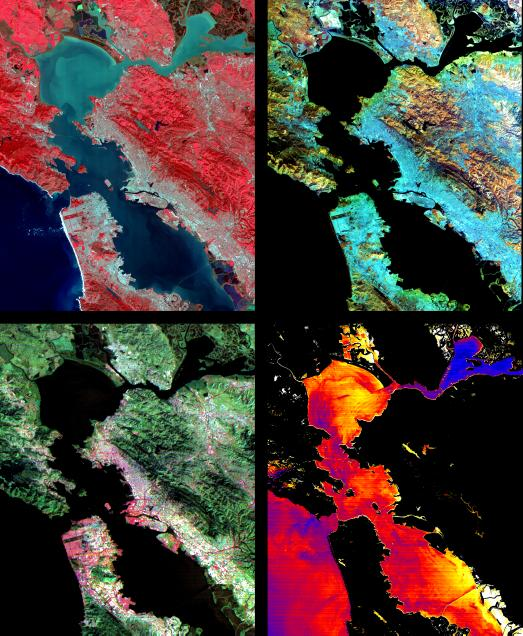
\includegraphics[width=3.78125in,height=\textheight]{images/PIA02605_modest.jpg}}

\end{figure}

Figure 1 : ASTER images of San Fransisco. source :
\href{https://photojournal.jpl.nasa.gov/catalog/PIA02605}{NASA/JPL}

For example, see the ASTER images of San Fransisco Bay above it
highlights different object such as vegetation (upper left); soil \&
rocks in mountainous area (upper right); urban materials (lower left) ;
and water temperature (lower right).

Practically, learning this course will, hopefully, help me address the
challenges I faced during my previous work in Indonesia. For example,
while working on a project focused on healthcare accessibility across
hundreds of small islands, we struggled to obtain real-time data to
identify which islands were inhabited and which were not. Additionally,
we faced challenges in determining which islands had ports suitable for
docking ships. I believe that applying remote sensing data is both cost-
and time-efficient in helping the government maintain more precise and
up-to-date data, which is particularly important in world's largest
archipelago country like Indonesia.

Feel free to explore my site to learn more about my learning experience.
Hope it helps!

\bookmarksetup{startatroot}

\hypertarget{getting-to-know-remote-sensing}{%
\chapter{Getting to Know Remote
Sensing}\label{getting-to-know-remote-sensing}}

\hypertarget{summary}{%
\section{\texorpdfstring{\textbf{Summary}}{Summary}}\label{summary}}

This week the lecture covers an introduction of remote sensing is, such
as its vast application, instruments, collection method, and things we
have to consider when we deal with remote sensing data. I tried to make
the summary using visualization below to make it easier to understand.

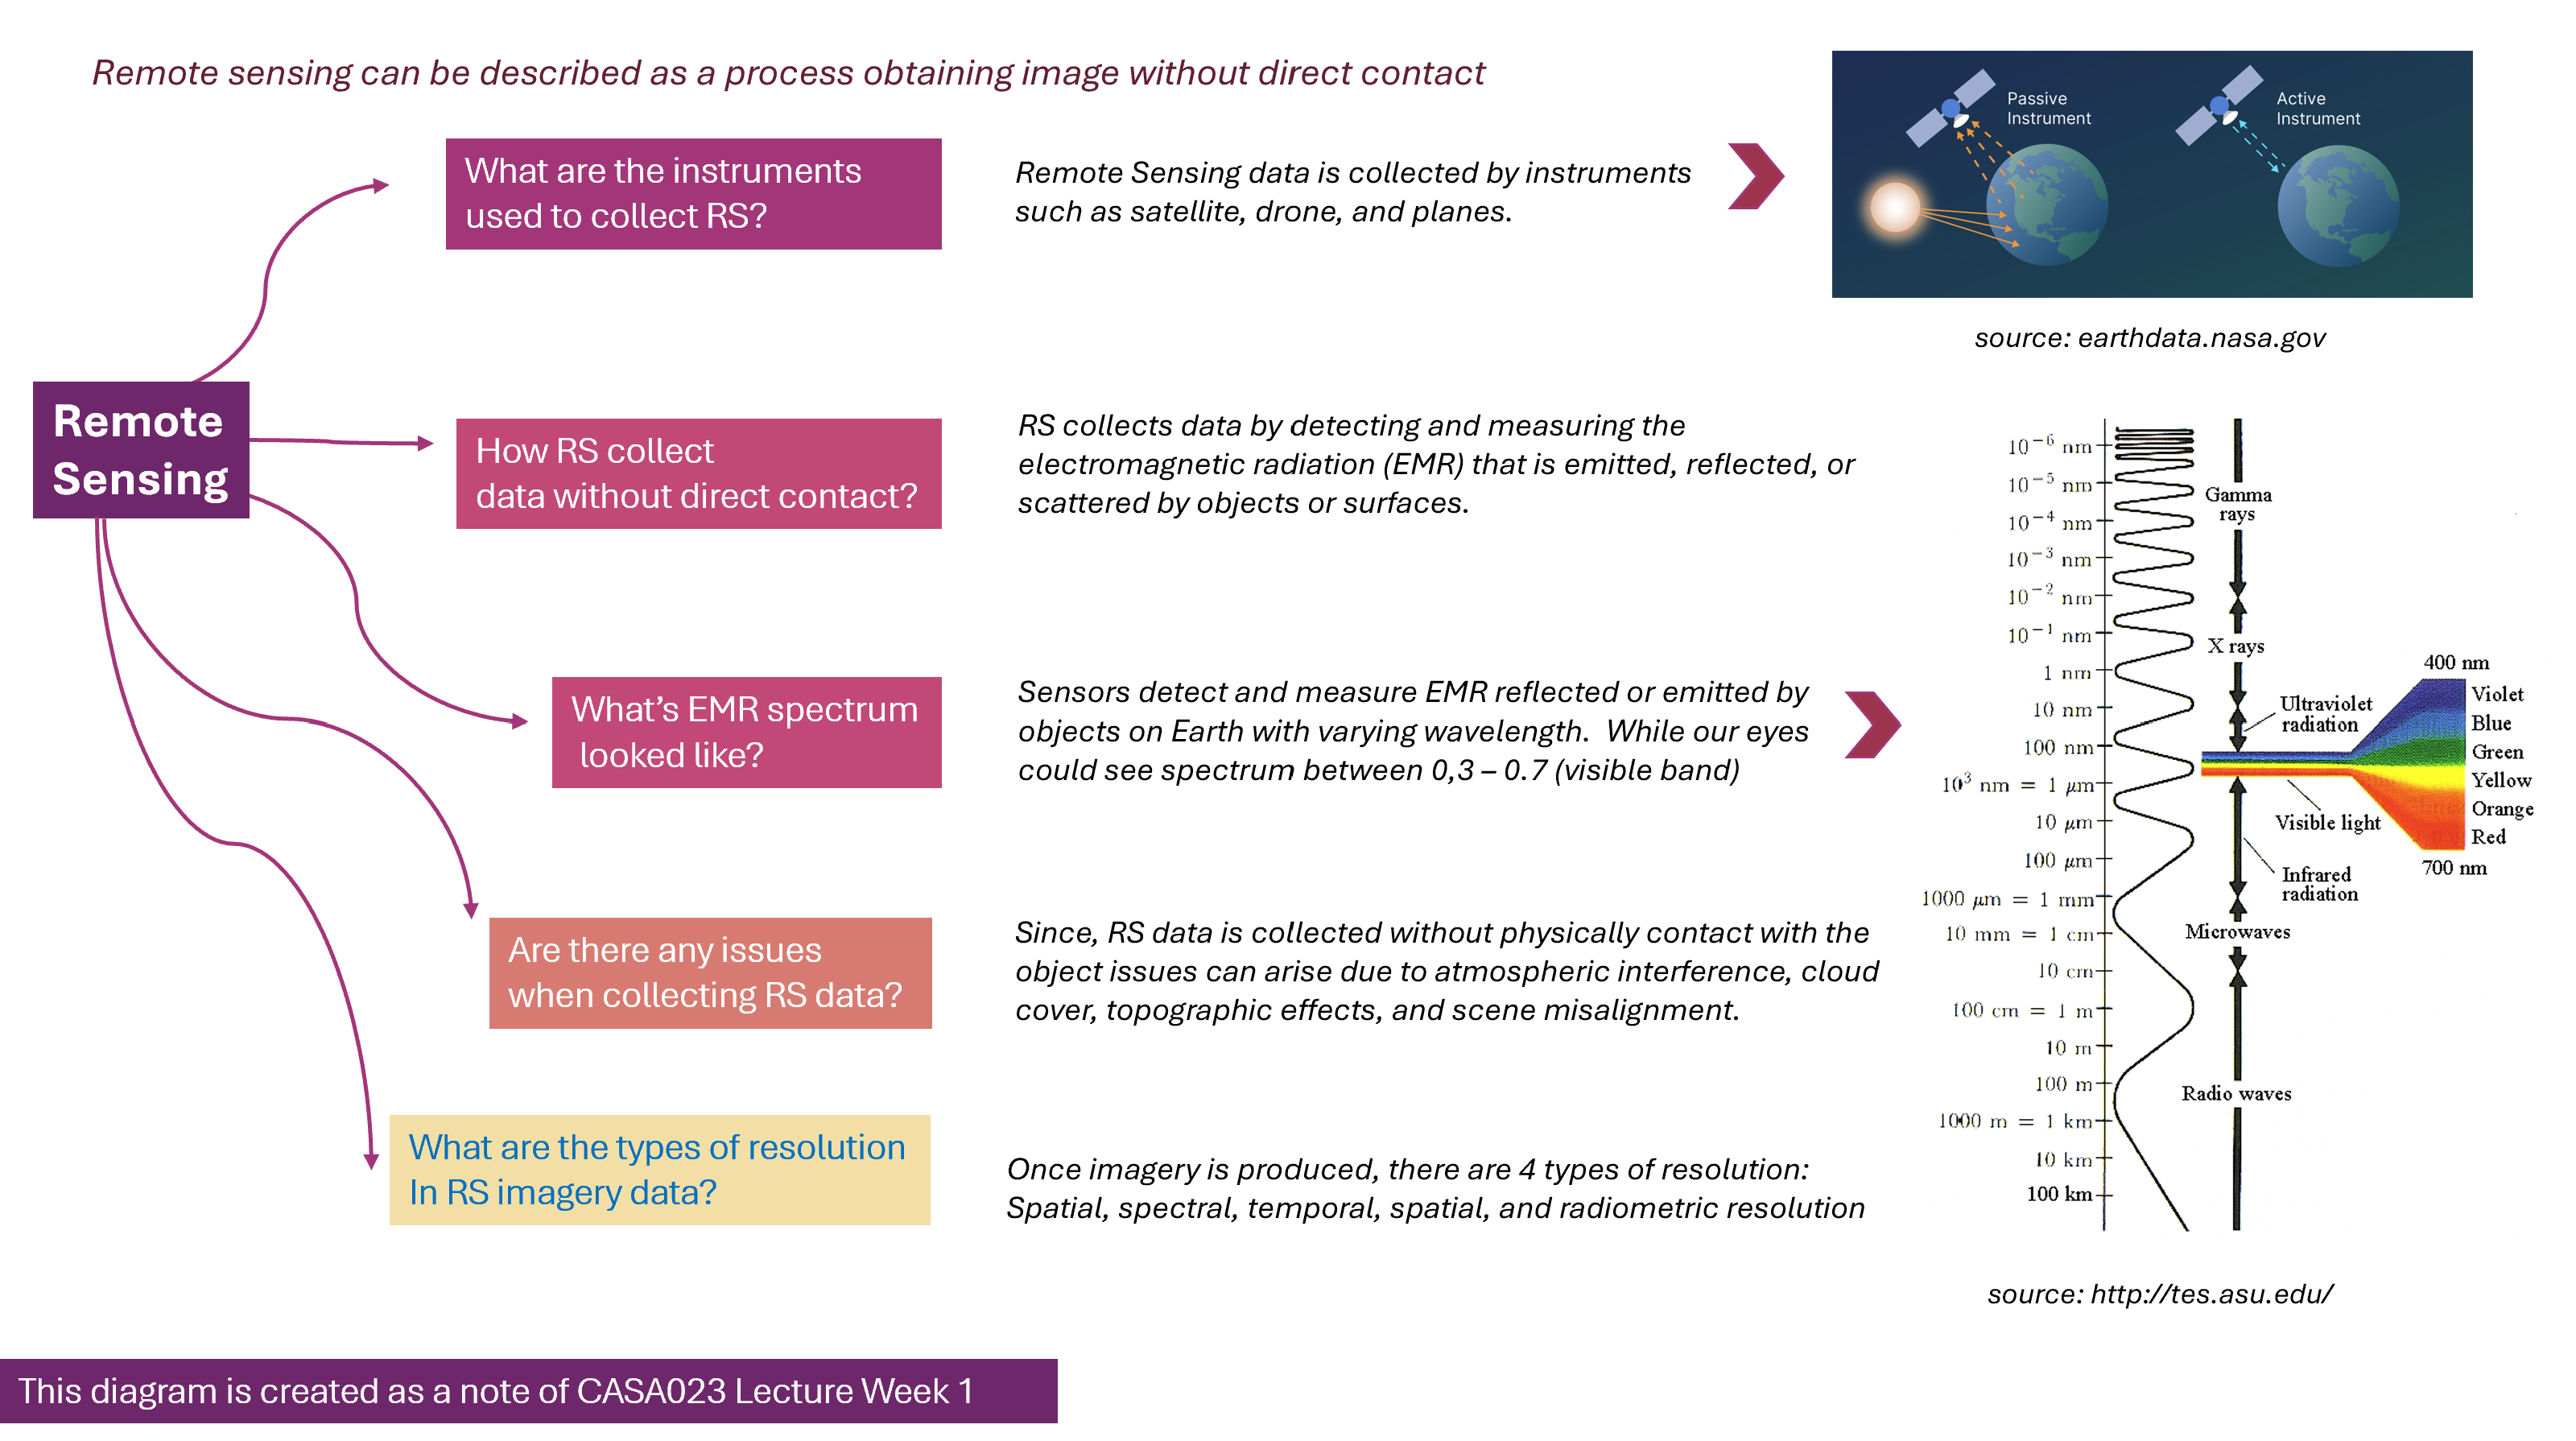
\includegraphics{images/clipboard-1084697230.png}

During the practical, we explore several tools to deal with remote
sensing data such as SNAP (Sentinel Application Platform) and R-studio
to plot spectral signature. We are also introduced with 2 imagery :
Sentinel-2A and Landsat-8. It is interesting how this two imagery has a
global coverage and for FREE. Both of them has spectral bands that could
be useful for vegetation monitoring, land cover classification, and
agricultural applications. We could benefit from Sentinel-2 frequent
observations to monitor rapid changes. Meanwhile, Landsat data allows us
to do large areas and long-term vegetation monitoring as it has
extensive historical archive and consistent global coverage. Below I
discussed the application of both Landsat and Sentinel in a vegetation
analysis.

\hypertarget{application}{%
\section{\texorpdfstring{\textbf{Application}}{Application}}\label{application}}

\begin{quote}
\textbf{Landsat for monitoring accross vast region : Detecting of
vegetation evolution across China Urban Development}
\end{quote}

\begin{itemize}
\item
  Han et al. (2025) explores 30 years of landsat archive data (spanning
  of landsat 5 to 8) on 2.125 city to monitor the vegetation evolution,
  using reflective bands such as Blue, green, red, NIR and SWIR (1 and
  2) and highlighting vegetation characteristics using NDVI, EVI, and
  OSAVI. The NDVI and RGB bands were further processed to derive texture
  variables, including variance, contrast, entropy, angular second
  moment, and correlation. These texture metrics capture spatial
  patterns and fine-scale structural details of urban vegetation that
  may not be visible through spectral bands alone. The findings will
  classify vegetation in urban area, whether it is decreasing or
  increasing over time. I genuinely believe this finding has the
  potential to serve as a framework for evaluating the effectiveness of
  the government's long-term plan on urban greening. For instance in my
  country, Indonesia we have long-term regional planning that spanning
  for 20 years (reviewed every 5 years), the analyisis will help the
  policy maker to formulate more measured-target.

  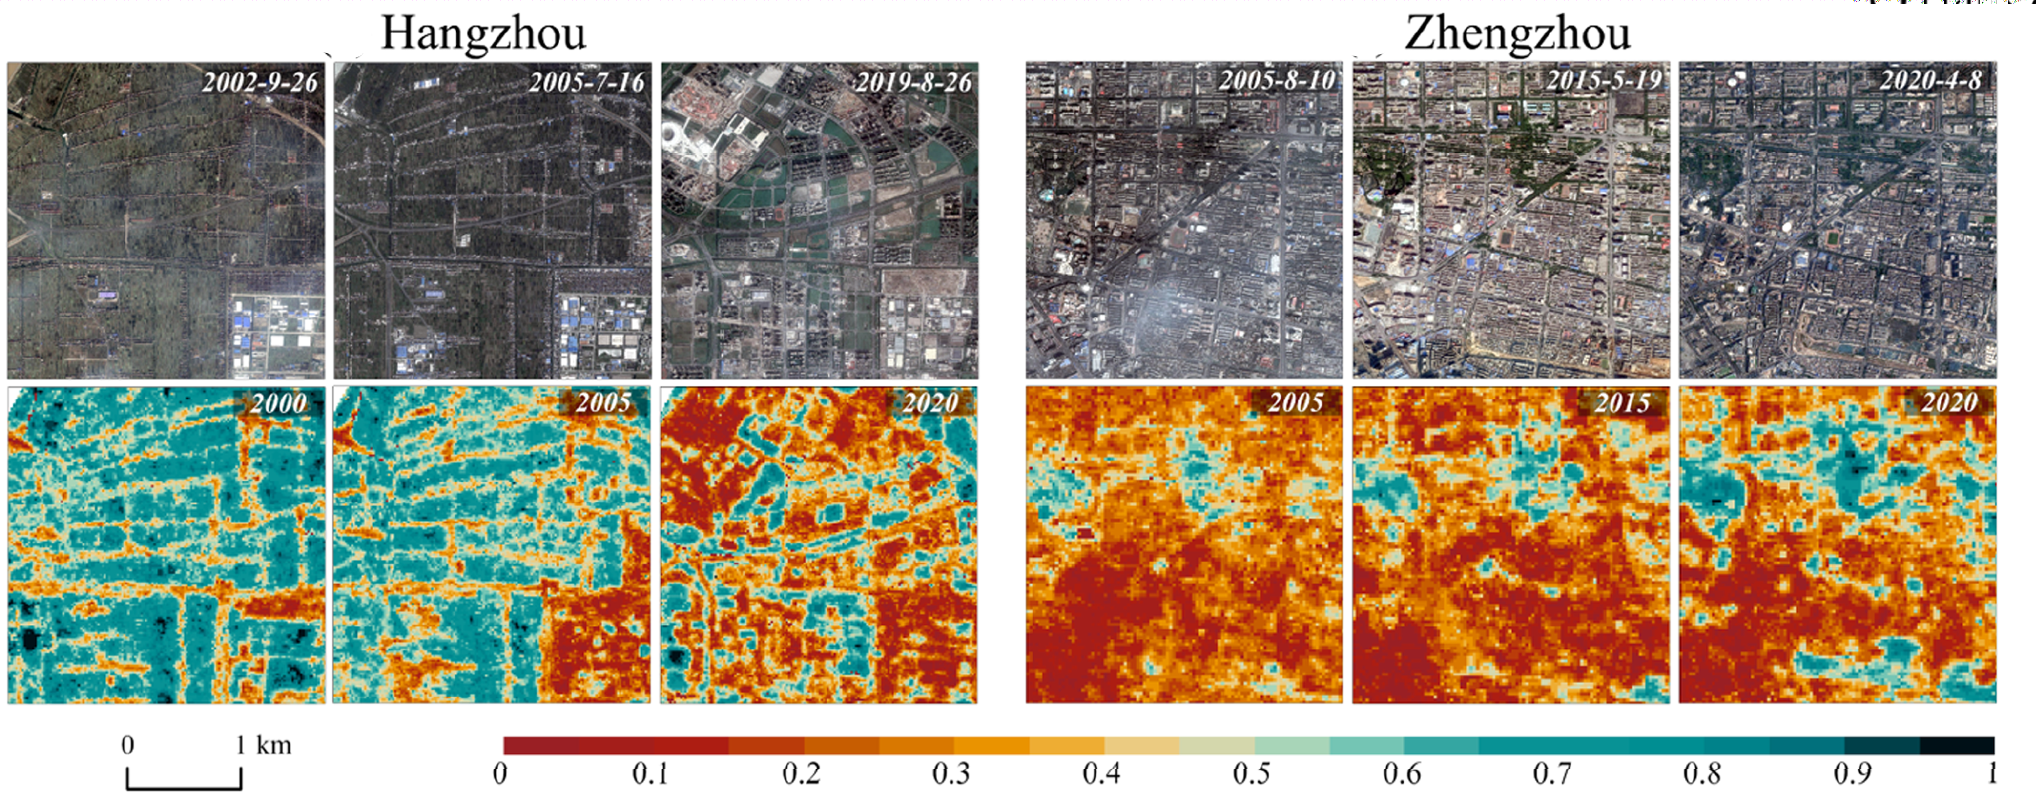
\includegraphics[width=6.96875in,height=\textheight]{images/clipboard-1072383063.png}

  Figure 1: A sample result shows urban vegetation degradation in
  Hangzhou and an increase in vegetation in Zhengzhou. source : (Han et
  al. 2025).
\end{itemize}

However, Landsat is an optical imaging system that is often susceptible
to cloud cover and has limitations in distinguishing different
vegetation types based solely on spectral characteristics. Imagine
studying a mountainous region where cloud cover is persistent---using
optical images like Landsat for vegetation monitoring and identification
would be challenging.

To address this issue, Li et al.~(2023) utilized Sentinel-1, which
operates with C-band Synthetic Aperture Radar (SAR), enabling vegetation
mapping under all weather conditions. The SAR data from Sentinel-1, when
combined with the optical imagery of Sentinel-2, allows for the
production of high-resolution maps that effectively differentiate bamboo
forests from other vegetation types. This integration helps overcome the
limitations of optical data in vegetation monitoring, where mixed
spectral characteristics often lead to uncertainty in distinguishing
bamboo from other forest types.

\hypertarget{reflection}{%
\section{Reflection}\label{reflection}}

After exploring the application of the two selected satellites, I have
concluded that remote sensing data is particularly effective for
analyzing large-scale and long-term variations. It can also help
mitigate the high costs of manual data collection across vast regions.
This insight made me reflect on a similar challenge in my country,
Indonesia. We often have challenges to find datasets for spatial
analysis as we rely much on vector data, if any it would be outdated.
Using remote sensing data not only allows us to have more updated data
but also allows us to explore various potential variables derived from
satellite imagery.

\hypertarget{references}{%
\section{References}\label{references}}

\bookmarksetup{startatroot}

\hypertarget{xaringan-and-quarto-book}{%
\chapter{Xaringan and Quarto Book}\label{xaringan-and-quarto-book}}

Lecture this week reminded me of one of powerful figure in Uchiha Clan,
the one who can manipulate reality once he activates this-so-called
Xaringan. Well, but this Xaringan is not related to figures in Konoha's
world but related to a certain library in R Studio that enable us to
create neat HTML slides in R.

\hypertarget{summary-1}{%
\section{Summary}\label{summary-1}}

\begin{Shaded}
\begin{Highlighting}[]
\NormalTok{xaringanExtra}\SpecialCharTok{::}\FunctionTok{embed\_xaringan}\NormalTok{(}\AttributeTok{url =} \StringTok{"https://nooriza16.github.io/Xaringan/Xaringan.html"}\NormalTok{, }\AttributeTok{ratio =} \StringTok{"16:9"}\NormalTok{)}
\end{Highlighting}
\end{Shaded}

\hypertarget{reflections}{%
\section{Reflections}\label{reflections}}

For someone who is not familiar with html, learning Xaringan is
definitely challenging compared to powerpoint, as we just usually click
tabs on power point. Honestly, I still consider power point provides
more themes and more visualization effects that is easily to access
compared to Xaringan. However, as I delved further I realize that using
Xaringan is providing us with flexibility even such as positioned our
picture.

So far, I feel like Xaringan is best at incorporating snippet code on
presentation or interactive features that usually too heavy to load in
power point. Besides, it helps me to give a sense of what html look
like.

\bookmarksetup{startatroot}

\hypertarget{image-correction}{%
\chapter{Image Correction}\label{image-correction}}

\hypertarget{summary-2}{%
\section{Summary}\label{summary-2}}

\hypertarget{application-1}{%
\section{Application}\label{application-1}}

\hypertarget{reflections-1}{%
\section{Reflections}\label{reflections-1}}

I think performing Remote Sensing correction on R Studio is quite
challenging, as I become more used to using `button' in Remote Sensing
application such as ENVI or SNAP. Besides, after this week's lecture, I
genuinely think that Remote Sensing is quite complex as it is not only
an image but behind the imagery each pixel is composed by digital number
collection and it could be linked with regression too !

\bookmarksetup{startatroot}

\hypertarget{policy}{%
\chapter{Policy}\label{policy}}

\textbf{Project Case : A New Relocated Capital City of Indonesia ; From
Jakarta to Nusantara}

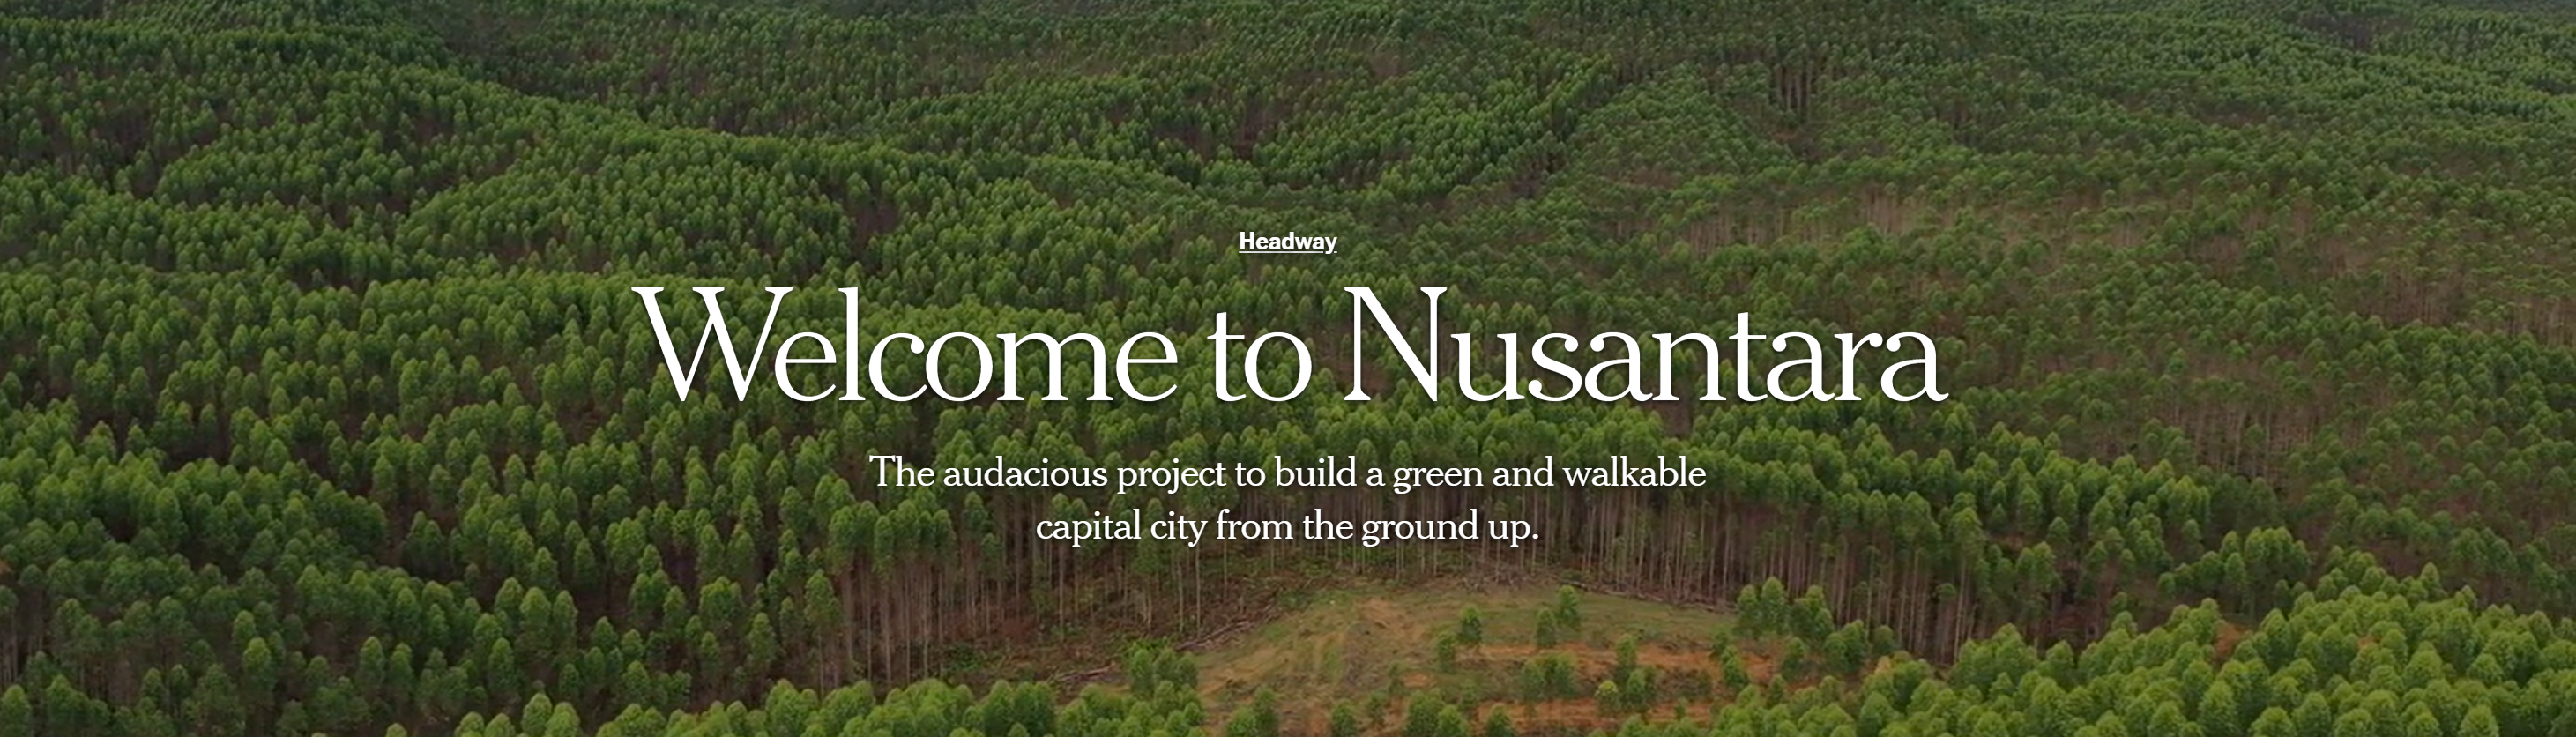
\includegraphics[width=9.82292in,height=\textheight]{images/clipboard-546673402.png}

Source :
\href{https://www.nytimes.com/interactive/2023/05/16/headway/indonesia-nusantara-jakarta.html}{www.nytimes.com}

\hypertarget{summary-3}{%
\section{Summary}\label{summary-3}}

Recently Indonesia planned to move its capital city from Jakarta (in
Java islands) into Penajam Paser Utara City (Borneo Islands), as the
current capital city, Jakarta, faced an issue of sinking, land
subsidence, overcrowding, low air and water quality (Bappenas 2021). The
term Nusantara is used to name this new capital city, symbolizing the
varied geographic settings and cultural diversities of Indonesia.

As for the time this published, Nusantara Development is on the phase 2
(2025-2029) that involved strengthening core area (housing, office,
commercial zone). Thus, in the time being, Jakarta will still remain the
capital of Indonesia until the Presidential Decree on the transfer of
the capital to Nusantara is issued. The issuance of this decree will
depend on the readiness of the new capital city, including the
preparation of all supporting systems such as infrastructure, human
resources, and governance systems.

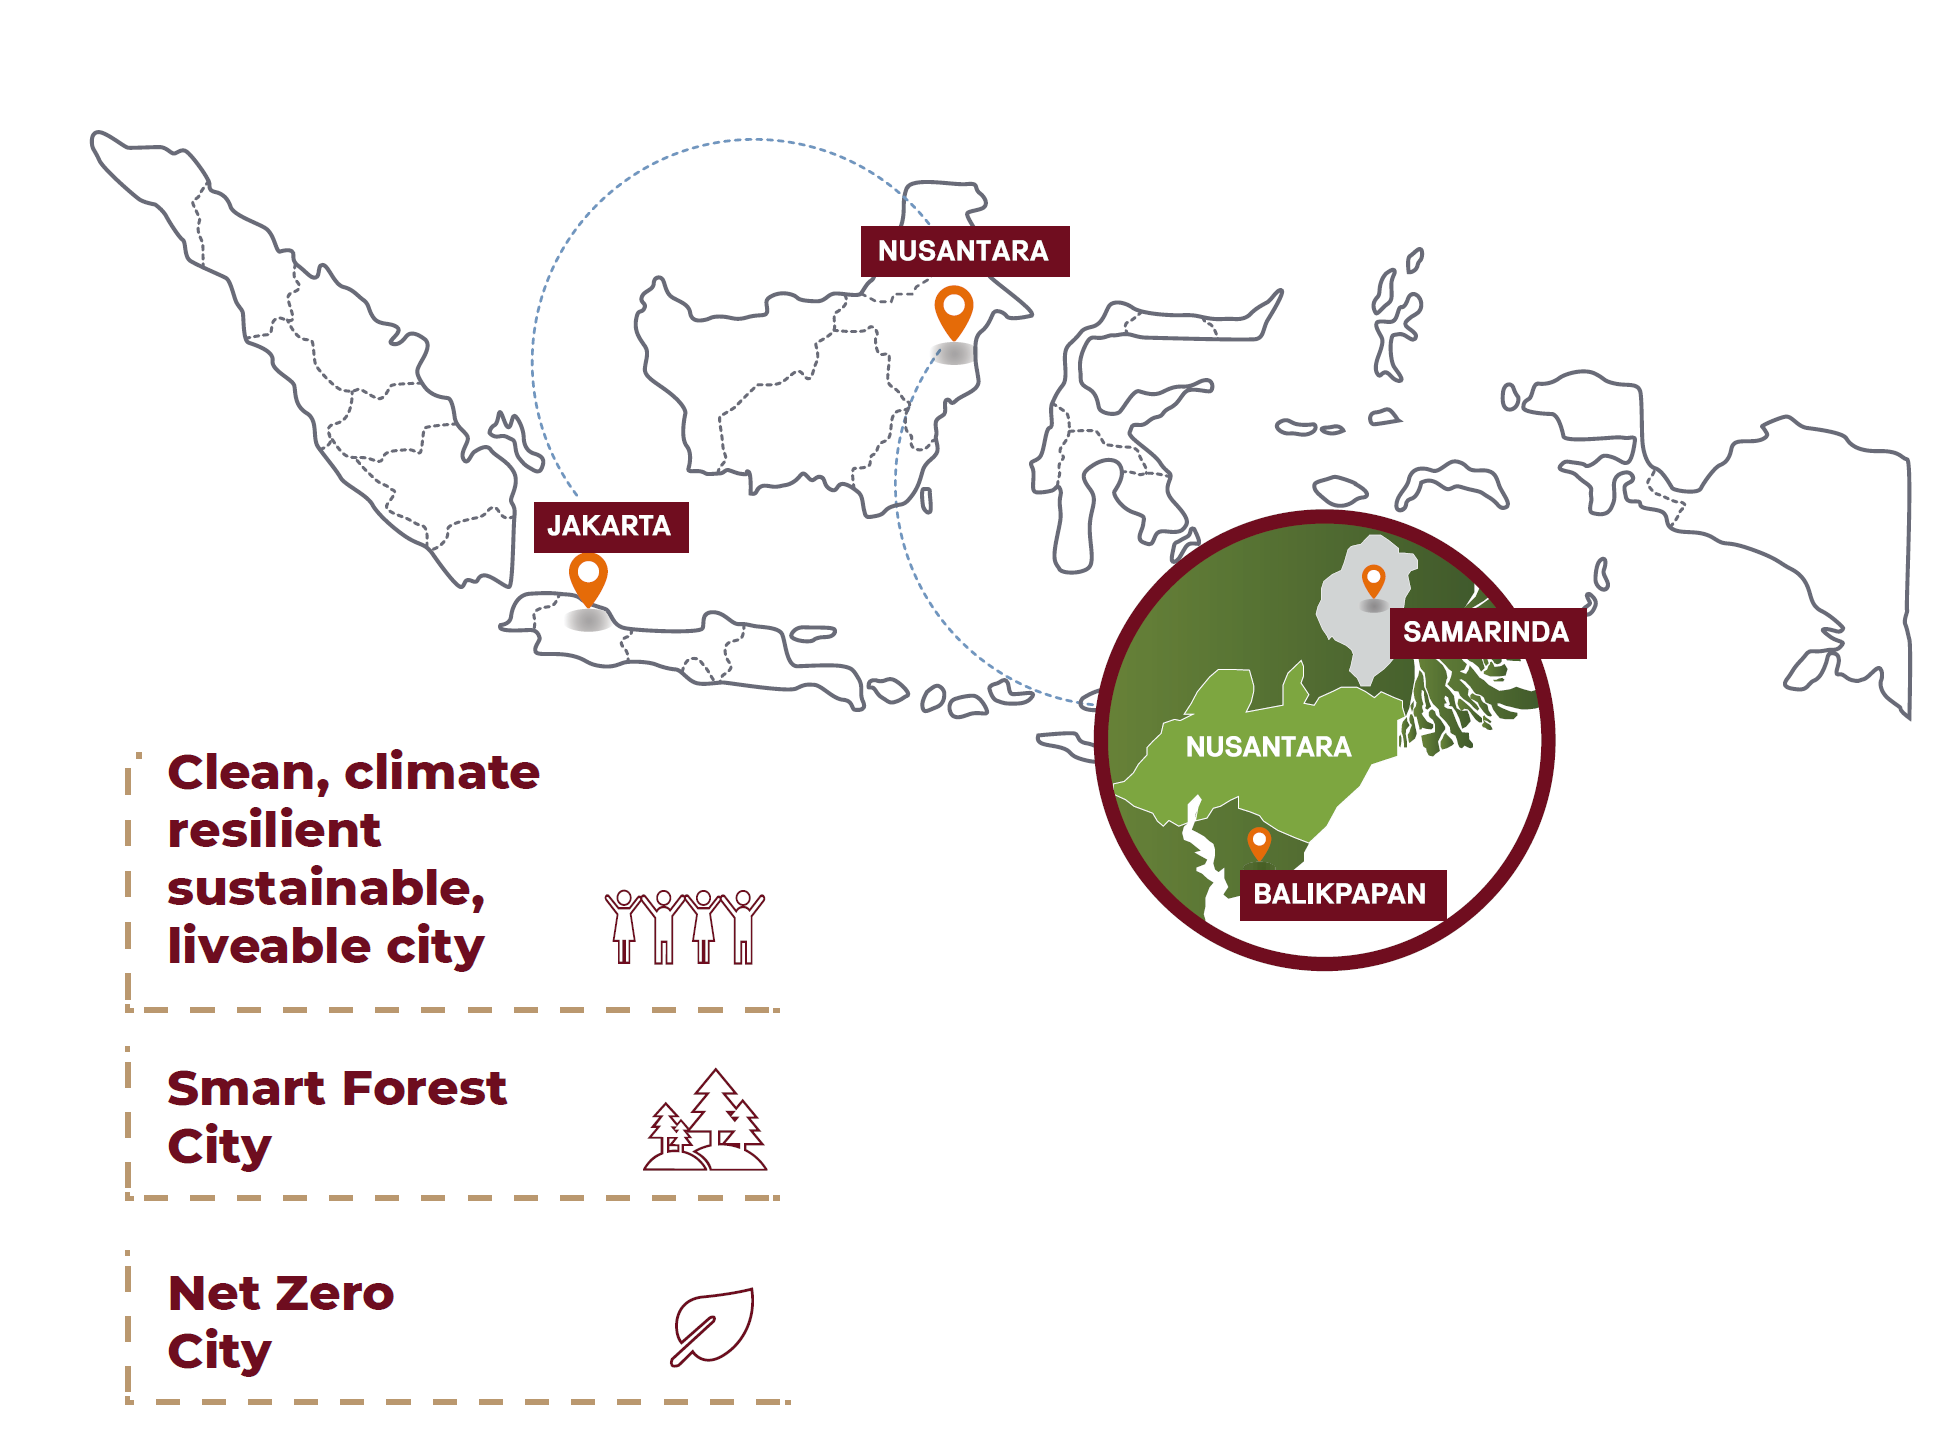
\includegraphics[width=6.07292in,height=\textheight]{images/clipboard-3462147358.png}

Figure 1: The Relocation Settings and Vision. source: (Capital Authority
2024)

As the development is still in the initial stage, the detailed planning
documents haven't been launched yet. Thus, I use available published
documents regarding the detail of Nusantara's Development which all of
them are publicly available, such as:

\begin{enumerate}
\def\labelenumi{\arabic{enumi}.}
\tightlist
\item
  \href{https://www.ikn.go.id/storage/pedoman-nusantara/2/nusantara-vlr-baseline-en.pdf}{Nusantara
  Sustainable Development Goals (SDGs) Voluntary Local Review Baseline
  {[}2024{]}}
\item
  \href{https://ikn.go.id/storage/pedoman-nusantara/1/nusantara-biodiversity-management-master-plan-2024.pdf}{Nusantara
  Biodiversity Management Master Plan} {[}2024{]}
\end{enumerate}

\begin{quote}
\textbf{Policy}
\end{quote}

The new capital city, Nusantara, is designed as a \textbf{forest city},
with 75\% of its designated area being green space. This design aims to
create a harmonious blend of urban development and biodiversity hotspots
(Borneo Island, where Nusantara is located, is famous for its tropical
rainforests). However, the design of being a forest city, its proximity
to the rainforest, and its drive on landscape change would present
significant \textbf{challenges}. One of the major concerns is the
increasing likelihood of mosquito-borne diseases (such as
\textbf{malaria}) spreading in the new capital, which are prevalent in
tropical regions Surendra et al. (2024).

Since malaria is both a global and local challenge, certain goals should
be considered to support Nusantara's sustainability, such as:

\textbf{A. Global Goals :} Sustainable Development Goals (SDGs) 3.3 :
Fight Communicable Diseases

The SDGs propose achievable global in combating malaria with target that
in include reducing incident, mortality rates, eliminate malaria in 35
countries by 2030 and prevent resurgence of the disease in a
malaria-free country. Meanwhile, Indonesia's estimated malaria incidence
per 1000 population at risk is still on range between 1-50 incidents per
1000 population in 2023. To achieve target of Global Goals, (WHO 2021)
have launched global technical strategy for malaria with framework such
as:

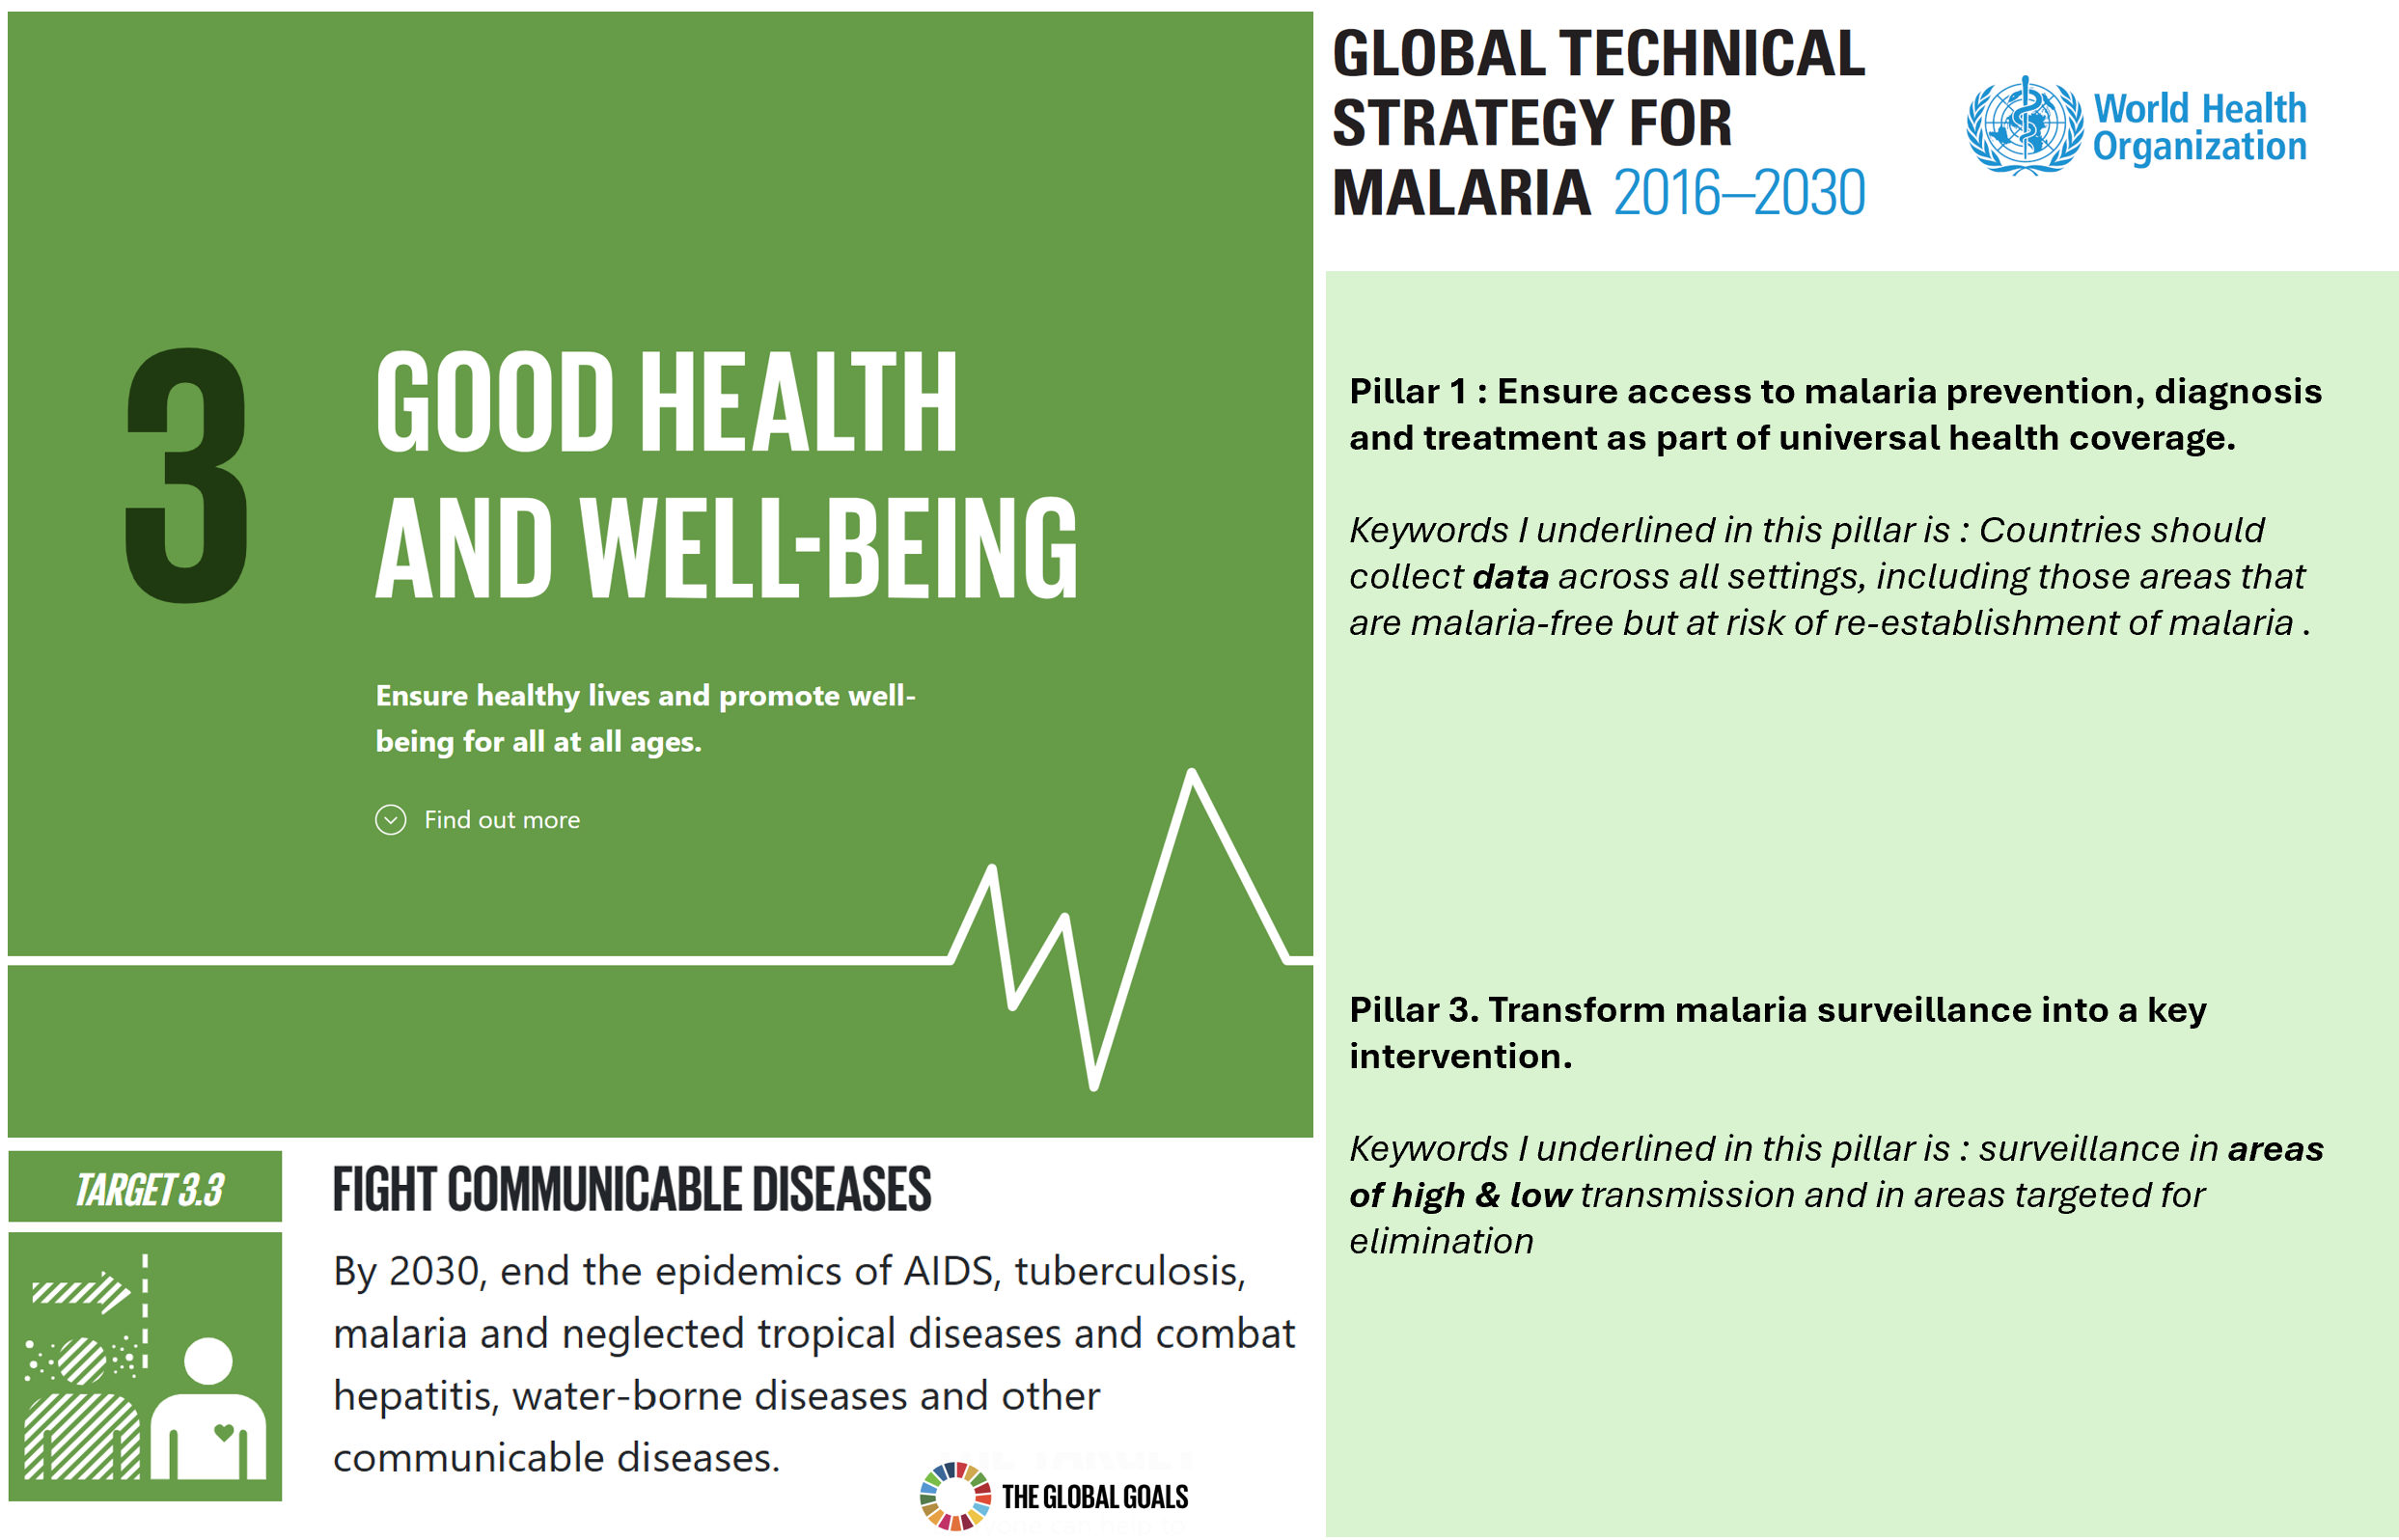
\includegraphics[width=7.76042in,height=\textheight]{images/clipboard-2410472720.png}

Figure 2 : SDGs Goal and WHO Technical Strategy

\textbf{B. Local Goals (National Level):} Eliminate malaria case by 2030
and maintain malaria free status

Translating the global goals on malaria elimination, Indonesia's
Ministry of Health (Ministry of Health and Control 2023) had proposed
recommendations, including the new capital city such as:

\begin{itemize}
\item
  Malaria elimination policies and implementation need basic research,
  operational support, and efficient technology development.
\item
  Provide input to the IKN special authority regarding malaria risk to
  ensure the design of the IKN area drainage system is free from malaria
  mosquito larvae habitat
\item
  Mapping legal and illegal forest encroachers to develop an activity
  plan and budget
\end{itemize}

\hypertarget{application-2}{%
\section{Application}\label{application-2}}

\begin{quote}
Remote Sensing as Baseline for detecting malaria hotspot
\end{quote}

In malaria elimination projects, remote sensing can serve as a crucial
baseline data source for mapping malaria hotspots by integrating
climatic and land-use factors. @wimberly2021 proposed a framework that
leverages Earth observation products to identify mosquito habitats based
on climate conditions, human activities, and specific land-use patterns.

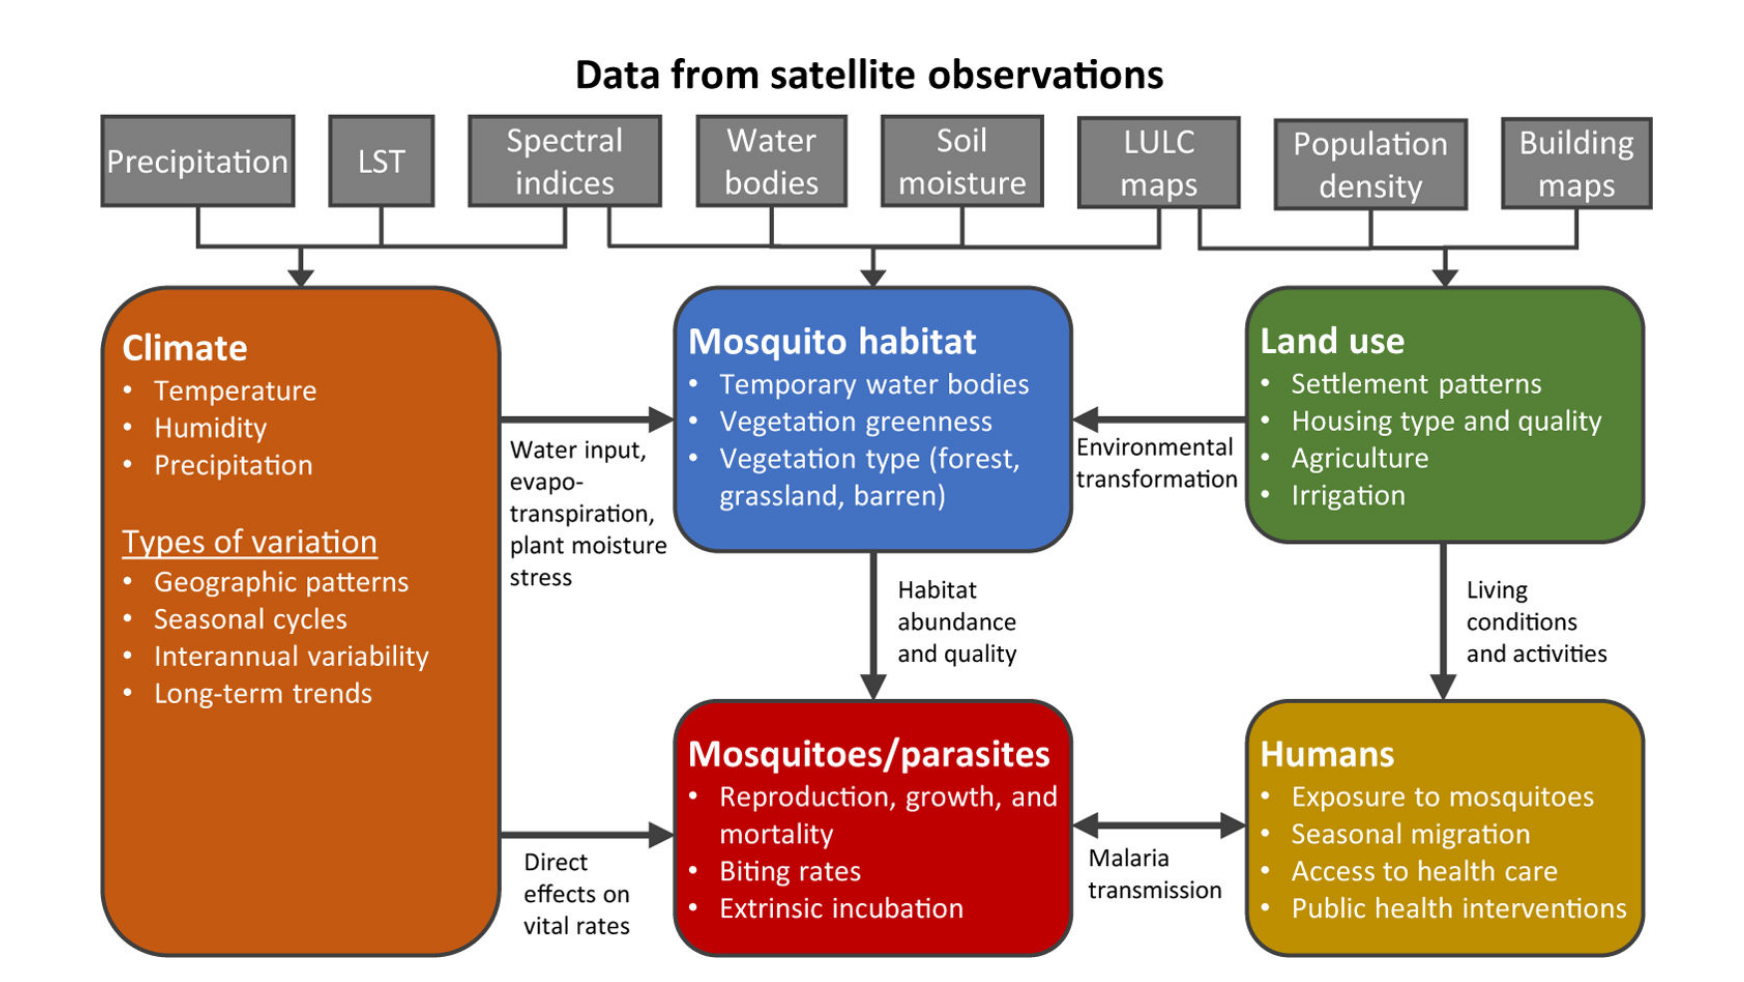
\includegraphics[width=7in,height=\textheight]{images/clipboard-687725868.png}

Figure 2: Framework in which Remote Sensing used in Malaria studies.
source : Wimberly et al. (2021).

To address policy mentioned in section 2, I underlined some dataset that
could be used to the analysis:

\begin{itemize}
\item
  \textbf{Sentinel-2 (rainy season)}

  \begin{itemize}
  \item
    \emph{Highlight water bodies and wetlands} -- These serve as proxies
    for mosquito breeding sites.
  \item
    \emph{Vegetation and land cover} -- Provides insight into potential
    mosquito habitats.
  \item
    \emph{Surface temperature} -- Acts as a proxy for mosquito activity.
  \end{itemize}
\end{itemize}

\begin{itemize}
\item
  \textbf{Digital Elevation Model (DEM) Data/Topography}

  \begin{itemize}
  \tightlist
  \item
    Helps identify potential inundation areas, which could influence
    mosquito breeding patterns.
  \end{itemize}
\item
  \textbf{Microsoft Open Buildings}

  \begin{itemize}
  \tightlist
  \item
    Useful as a proxy for human settlements and potential exposure risk.
  \end{itemize}
\item
  \textbf{Rainfall Data}

  \begin{itemize}
  \tightlist
  \item
    The rainfall season can be considered as a timeframe for analysis.
    However, if locally recorded rainfall data from the Indonesian
    Climatic Institution is available, it could help refine the
    identification of rainfall patterns, allowing for a more informed
    selection of the time series.
  \end{itemize}
\end{itemize}

\hypertarget{reflections-2}{%
\section{Reflections}\label{reflections-2}}

During this week, I got a lot of reflections as I finally found lecture
that explicitly bridging the gap of `academics' to real-world policy. My
reflections would be:

\begin{quote}
\begin{enumerate}
\def\labelenumi{\arabic{enumi}.}
\tightlist
\item
  Combining remote sensing with GIS
\end{enumerate}
\end{quote}

Since Nusantara is still uninhabited, we could model nearby settlements
to investigate the remote sensing framework. By combining the results
with \textbf{malaria incident data}, we can validate our
classification---analyzing what percentage of high-risk areas have
recorded incidents and which have not. While global and local malaria
elimination frameworks mention aggregating incident data and risk
levels, they do not explicitly emphasize mapping. Using maps, we can
overlay malaria hotspots with incident data, land use, and
socio-economic factors. As (Naserrudin, Yong, et al. 2023) notes, people
are exposed to malaria due to professions that require them to venture
deeper into the forest.

\begin{quote}
\begin{enumerate}
\def\labelenumi{\arabic{enumi}.}
\setcounter{enumi}{1}
\tightlist
\item
  Remote Sensing and GIS is good, but enriching the analysis with
  \textbf{affected communities} make it better
\end{enumerate}
\end{quote}

Beyond remote sensing data, incorporating local knowledge can improve
the analysis. Understanding how affected communities respond to malaria
provides insight into the effectiveness of mitigation efforts
(Naserrudin, Lin, et al. 2023). These communities have lived near
rainforests for generations and are directly affected, making their
experiences valuable for practical prevention strategies..

\begin{quote}
\begin{enumerate}
\def\labelenumi{\arabic{enumi}.}
\setcounter{enumi}{2}
\tightlist
\item
  Implementation challenges, the need for collaboration
\end{enumerate}
\end{quote}

One the most important key-takeaway from the lecture is that ``some
academics papers are too technical, without clearly addressed policy;
some policy don't include academic findings they could benefit for.''
This condition lead to a gap between academics and urban governance.
However, in my observation during my work with the government the
potential cause is human resources (make the adoption of academics
finding hard to implement), annual budget cycles (governments prioritize
immediate results and may be reluctant to invest in the long-term
experimental processes typical of academia). Bridging the gap on malaria
prevention requires collaboration and commitment not only between
epidemiologists, healthcare, and geospatial analysts but with the
governments to ensure research translates into actionable policies.

\hypertarget{references-1}{%
\section*{References}\label{references-1}}
\addcontentsline{toc}{section}{References}

\hypertarget{refs}{}
\begin{CSLReferences}{1}{0}
\leavevmode\vadjust pre{\hypertarget{ref-bappenas2021}{}}%
Bappenas, Kementrian PPN. 2021. {``Buku Saku Pemindahan Ibu Kota
Negara.''}

\leavevmode\vadjust pre{\hypertarget{ref-capitalauthority2024}{}}%
Capital Authority, Nusantara. 2024. {``Nusantara Sustainable Development
GOals (SDGs) Voluntary Local Review Baseline.''}

\leavevmode\vadjust pre{\hypertarget{ref-han2025}{}}%
Han, Yuan, Jianhua He, Xiaoping Du, Xiao Han, and Yaolin Liu. 2025.
{``Reconstructing Urban Vegetation Evolution in China Using Multimodal
Deep Learning and 30-Years Landsat Archive.''} \emph{Urban Forestry \&
Urban Greening} 103 (January): 128582.
\url{https://doi.org/10.1016/j.ufug.2024.128582}.

\leavevmode\vadjust pre{\hypertarget{ref-ministryofhealth2023}{}}%
Ministry of Health, Directorate General of Disease Prevention, and
Control. 2023. {``National Action Plan for Acceleration of Malaria
Elimination 2020-2026 (Revision).''}
\url{https://malaria.kemkes.go.id/sites/default/files/2024-08/National\%20Strategic\%20Plan\%20Revision_Malaria_29\%20Mei\%202023.pdf}.

\leavevmode\vadjust pre{\hypertarget{ref-naserrudin2023a}{}}%
Naserrudin, Nurul Athirah, Pauline Yong Pau Lin, April Monroe, Richard
Culleton, Sara Elizabeth Baumann, Shigeharu Sato, Bipin Adhikari, et al.
2023. {``Exploring Barriers to and Facilitators of Malaria Prevention
Practices: A Photovoice Study with Rural Communities at Risk to
Plasmodium Knowlesi Malaria in Sabah, Malaysia.''} \emph{BMC Public
Health} 23 (1): 1316. \url{https://doi.org/10.1186/s12889-023-16173-x}.

\leavevmode\vadjust pre{\hypertarget{ref-naserrudin2023}{}}%
Naserrudin, Nurul Athirah, Pauline Pau Lin Yong, April Monroe, Richard
Culleton, Sara Elizabeth Baumann, Shigeharu Sato, Rozita Hod, Mohammad
Saffree Jeffree, Kamruddin Ahmed, and Mohd Rohaizat Hassan. 2023.
{``Seeing Malaria Through the Eyes of Affected Communities: Using
Photovoice to Document Local Knowledge on Zoonotic Malaria Causation and
Prevention Practices Among Rural Communities Exposed to Plasmodium
Knowlesi Malaria in Northern Borneo Island.''} \emph{Malaria Journal} 22
(1): 166. \url{https://doi.org/10.1186/s12936-023-04603-5}.

\leavevmode\vadjust pre{\hypertarget{ref-surendra2024}{}}%
Surendra, Henry, Bimandra A. Djaafara, Helen D. Prameswari, Dedy
Supriyanto, Ponco Waluyo, Setyo B. Basuki, Herdiana Herdiana, et al.
2024. {``Mitigating Risks of Malaria and Other Vector-Borne Diseases in
the New Capital City of Indonesia.''} \emph{Nature Communications} 15
(1): 10575. \url{https://doi.org/10.1038/s41467-024-54891-x}.

\leavevmode\vadjust pre{\hypertarget{ref-who2021}{}}%
WHO, World Health Organization. 2021. {``Global Technical Strategy for
Malaria 2016{\textendash}2030, 2021 Update.''}

\leavevmode\vadjust pre{\hypertarget{ref-wimberly2021}{}}%
Wimberly, Michael C., Kirsten M. de Beurs, Tatiana V. Loboda, and
William K. Pan. 2021. {``Satellite Observations and Malaria: New
Opportunities for Research and Applications.''} \emph{Trends in
Parasitology} 37 (6): 525--37.
\url{https://doi.org/10.1016/j.pt.2021.03.003}.

\end{CSLReferences}



\end{document}
